\section{Definições dirigidas pela sintaxe}

\begin{frame}[fragile]{Definição dirigida pela sintaxe}

    \begin{block}{Definição}
        Uma definição dirigida pela sintaxe é uma generalização de uma gramática livre de contexto na qual cada símbolo gramatical
        possui um conjunto de atributos, particionados em dois subconjuntos: atributos herdados e atributos sintetizados.
    \end{block}

\end{frame}

\begin{frame}[fragile]{Atributos}

    \begin{itemize}
        \item Se cada nó da árvore gramatical contém um registro para armazenar informações, cada atributo seria um membro deste
            registro
        \pause

        \item Um atributo pode representar qualquer valor associado ao símbolo gramatical (um número, uma cadeia, um endereço de memória,
            etc)
        \pause

        \item O valor para um atributo de uma árvore gramatical é computado a partir de uma regra semântica associada à produção usada
            naquele nó
        \pause

        \item Um atributo sintetizado é computado a partir dos valores dos atributos dos filhos do nó
        \pause

        \item Um atributo herdado é computado a partir dos valores dos atributos dos irmãos e do pai do nó
    \end{itemize}

\end{frame}

\begin{frame}[fragile]{Regras semânticas}

    \begin{itemize}
        \item As regras semânticas estabelecem dependências entre os atributos, as quais são representadas por meio de um grafo
        \pause

        \item A ordem de avaliação das regras gramaticais é derivada a partir do grafo de dependências
        \pause

        \item A avaliação das regras semânticas determina os valores dos atributos para os nós da árvore gramatical para uma dada 
            cadeia de entrada
        \pause

        \item Regras semânticas podem ter efeitos colaterais associados
        \pause

        \item Na prática, a árvore semãntica ou o grafo de dependências não precisam ser construídos explicitamente
        \pause

        \item Uma árvore gramatical que exibe os valores dos atributos de cada nó é denominada árvore gramatical anotada
        \pause

        \item O processo de computador os valores dos atributos é denominado anotação da árvore
    \end{itemize}

\end{frame}

\begin{frame}[fragile]{Gramática de atributos}

    \begin{block}{Definição}
        Seja uma definição dirigida pela sintaxe. Cada produção $A\to \alpha$ estará associada a um conjunto de regras semânticas da
        forma $b := f(c_1, c_2, \ldots, c_k)$ onde $f$ é uma função, $c_1, c_2, \ldots, c_k$ são atributos pertencentes aos símbolos
        gramaticais da produção e vale apenas uma das duas alternativas:
        \begin{enumerate}[(i)]
            \item $b$ é um atributo sintetizado de $A$
            \item $b$ é um atributo herdado, pertencente ao um dos símbolos do lado direito da produção
        \end{enumerate}
        Em ambos casos, $b$ depende dos atributos $c_1, c_2, \ldots, c_k$.

        \vspace{0.1in}
        Se, para qualquer atributo $b$, a função $f$ não possui efeitos colaterais, então esta definição dirigida pela sintaxe é 
        denominada gramática de atributos.
    \end{block}

\end{frame}

\begin{frame}[fragile]{Exemplo de definição dirigida pela sintaxe}

    \begin{table}
        \centering
        \begin{tabular}{lp{2cm}l} 
        \toprule
        \textbf{Produção} & & \textbf{Regra semântica} \\
        \midrule
        $L\to E\ \textbf{n}$ & & \Call{imprimir}{$E.val$} \\
        \rowcolor[gray]{0.9}
        $E\to E_1\ \code{apl}{+}\ T$ & &  $E.val := E_1.val + T.val$ \\
        $E\to T$ & & $E.val := T.val$ \\
        \rowcolor[gray]{0.9}
        $T\to T_1\ \code{apl}{×}\ F$ & &  $T.val := T_1.val \times F.val$ \\
        $T\to F$ & & $T.val := F.val$ \\
        \rowcolor[gray]{0.9}
        $F\to (E)$ & & $F.val := E.val$ \\
        $F\to \textbf{digito}$ & & $F.val := \textbf{digito}.lexval$ \\
        \bottomrule
        \end{tabular}
    \end{table}

    \vspace{0.2in}
    Nesta definição dirigida pela sintaxe para uma calculadora, $L$ representa uma linha, \textbf{n} uma quebra de linha e o atributo $lexval$ do terminal
    \textbf{digito} é determinado pelo analisador léxico.
        
\end{frame}

\begin{frame}[fragile]{Atributos sintetizados}

    \begin{itemize}
        \item Na prática, os atributos sintetizados são usados extensivamente
        \pause

        \item Uma definição dirigida pela sintaxe que utilize exclusivamente atributos sintetizados é denominada uma definição 
            S-atribuída
        \pause

        \item Em uma árvore gramatical para uma definição S-atribuída, os valores dos atributos dos nós podem ser todos computados
        avaliando-se as regras gramaticais dos nós, a partir das folhas para a raiz
        \pause

        \item No exemplo anterior, todos os atributos da definição dirigida pela sintaxe são sintetizados

    \end{itemize}

\end{frame}

\begin{frame}[fragile]{Árvore gramatical anotada para a expressão \code{apl}{3×5+4n}}

    \begin{figure}
        \centering
        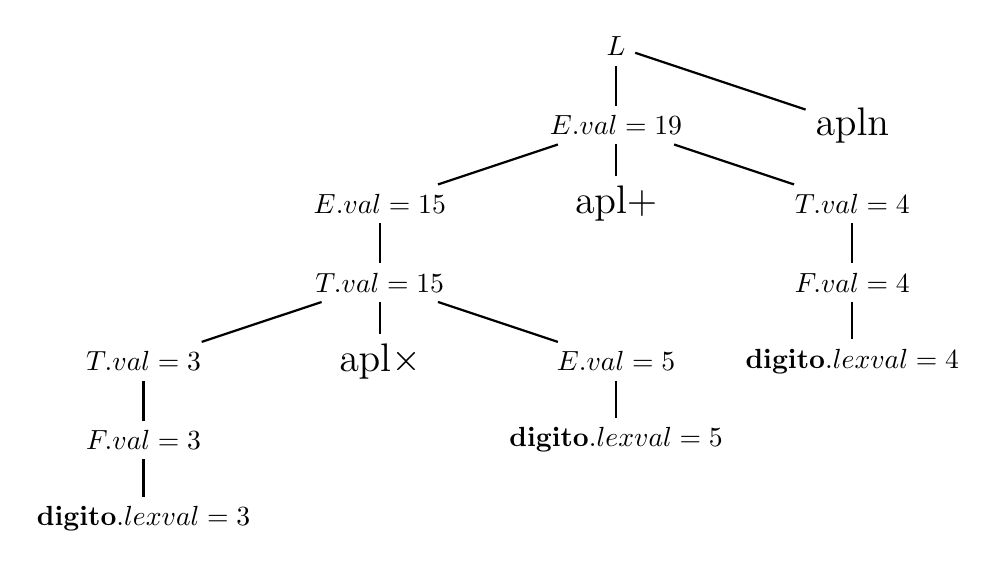
\begin{tikzpicture} 
            \node (A1) at (0, 2) { $T.val = 3$ };
            \node (A2) at (0, 1) { $F.val = 3$ };
            \node (A3) at (0, 0) { \textbf{digito}.$lexval = 3$ };

            \node (B1) at (3, 2) { \Large \code{apl}{×} };
            \node (B2) at (3, 3) { $T.val = 15$ };
            \node (B3) at (3, 4) { $E.val = 15$ };

            \node (C1) at (6, 6) { $L$ };
            \node (C2) at (6, 5) { $E.val = 19$ };
            \node (C3) at (6, 4) { \Large \code{apl}{+} };
            \node (C4) at (6, 2) { $E.val = 5$ };
            \node (C5) at (6, 1) { \textbf{digito}.$lexval = 5$ };

            \node (D1) at (9, 5) { \Large \code{apl}{n} };
            \node (D2) at (9, 4) { $T.val = 4$ };
            \node (D3) at (9, 3) { $F.val = 4$ };
            \node (D4) at (9, 2) { \textbf{digito}.$lexval = 4$ };

            \draw[thick] (A1) to (A2);
            \draw[thick] (A3) to (A2);
            \draw[thick] (B1) to (B2);
            \draw[thick] (A1) to (B2);
            \draw[thick] (B3) to (B2);
            \draw[thick] (B3) to (C2);
            \draw[thick] (C1) to (C2);
            \draw[thick] (C3) to (C2);
            \draw[thick] (C4) to (B2);
            \draw[thick] (C4) to (C5);
            \draw[thick] (C1) to (D1);
            \draw[thick] (C2) to (D2);
            \draw[thick] (D3) to (D2);
            \draw[thick] (D3) to (D4);
        \end{tikzpicture} 
    \end{figure}

\end{frame}

\begin{frame}[fragile]{Atributos herdados}

    \begin{itemize}
        \item Um atributo de um nó de uma árvore gramatical é dito herdado se o seu valor é definido a partir dos valores dos atributos
            de seu pai e/ou de seus irmãos
        \pause

        \item Tais atributos são úteis para representar relações de dependência de um construção de uma linguagem de programação com
            o contexto onde ele ocorre
        \pause

        \item Por exemplo, com atributos herdados é possível determinar se um identificador aparece do lado esquerdo ou direito de
            uma atribuição
        \pause

        \item É possível reescrever uma definição dirigida pela sintaxe de modo que sejam usados apenas atributos sintetizados
        \pause

        \item Contudo, o uso de atributos herdados permite uma descrição mais natural das relações de dependência
    \end{itemize}

\end{frame}

\begin{frame}[fragile]{Exemplo de definição dirigida pela sintaxe com atributo herdado}

    \begin{table}
        \centering
        \begin{tabular}{lp{2cm}l} 
        \toprule
        \textbf{Produção} & & \textbf{Regra semântica} \\
        \midrule
        \rowcolor[gray]{0.9}
        $D\to TL$ & & $L.in := T.tipo$ \\
        $T\to \textbf{int}$ & & $T.tipo = inteiro$ \\
        \rowcolor[gray]{0.9}
        $T\to \textbf{real}$ & & $T.tipo = real$ \\
        \multirow{2}{*}{$L\to L_1, \textbf{id}$} & & $L_1.in := L.in$ \\
        & & $\Call{incluirTipo}{\textbf{id}, entrada, L.in}$ \\
        \rowcolor[gray]{0.9}
        $L\to \textbf{id}$ & & $\Call{incluirTipo}{\textbf{id}, entrada, L.in}$ \\
        \bottomrule
        \end{tabular}
    \end{table}

    \vspace{0.2in}

    A definição dirigida pela sintaxe acima gera definições $D$ onde a palavra-chave \textbf{int} ou \textbf{real} precedem uma lista
        de identificadores. O atributo $L.in$ é herdado, enquanto que o atributo $T.tipo$ é sintetizado.
\end{frame}

\begin{frame}[fragile]{Árvore gramatical da definição \code{apl}{real id1, id2, id3}}

    \begin{figure}
        \centering

        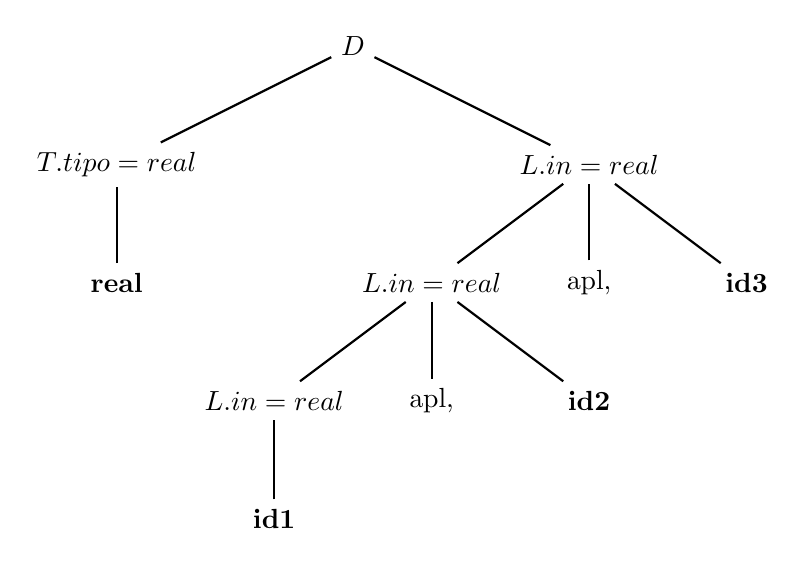
\begin{tikzpicture} 
            \node (A) at (6, 6) { $D$ };

            \node (B1) at (3, 4.5) { $T.tipo = real$ };
            \node (B2) at (9, 4.5) { $L.in = real$ };

            \node (C1) at (3, 3) { \textbf{real} };
            \node (C2) at (7, 3) {  $L.in = real$ };
            \node (C3) at (9, 3) {  \code{apl}{,} };
            \node (C4) at (11, 3) {  \textbf{id3} };

            \node (D1) at (5, 1.5) { $L.in = real$ };
            \node (D2) at (7, 1.5) { \code{apl}{,} };
            \node (D3) at (9, 1.5) { \textbf{id2} };

            \node (E1) at (5, 0) { \textbf{id1} };

            \draw[thick] (A) to (B1);
            \draw[thick] (A) to (B2);
            \draw[thick] (C1) to (B1);
            \draw[thick] (C2) to (B2);
            \draw[thick] (C3) to (B2);
            \draw[thick] (C4) to (B2);
            \draw[thick] (C2) to (D1);
            \draw[thick] (C2) to (D2);
            \draw[thick] (C2) to (D3);
            \draw[thick] (E1) to (D1);
        \end{tikzpicture} 
    \end{figure}

\end{frame}

\begin{frame}[fragile]{Grafo de dependências}

    \begin{block}{Definição}
        O grafo que estabelece as relações entre os diferentes atributos de uma definição dirigida pela sintaxe, onde os nós são
        os atributos e uma aresta $(a, b)$ indica que o atributo $a$ deve ser determinado antes do atributo $b$, é denominado
        grafo de dependências.
    \end{block}

    \vspace{0.2in}

    Na construção de um grafo de dependências, deve ser inserido um nó para cada chamada de procedimento, o que corresponde à
        introdução de um atributo fictício associado a esta chamada.

\end{frame}

\begin{frame}[fragile]{Algoritmo para geração do grafo de dependências}

    \begin{algorithmic}[1]
        \Require{Uma árvore gramatical de uma definição dirigida pela sintaxe}
        \Ensure{O grafo de dependência}

        \vspace{0.2in}

        \For{cada $n$ da árvore gramatical}
            \For{cada atributo $a$ do símbolo gramatical em $n$}
                \State{construa um nó no grafo de dependências para $a$}
            \EndFor
        \EndFor
        \Statex

        \For{cada $n$ da árvore gramatical}
            \For{cada regra semântica $b := f(c_1, c_2, \ldots, c_k)$ associada a produção usada em $n$}
                \For{$i = 1,k$}
                    \State{adicione ao grafo uma aresta partindo de $c_i$ para $b$}
                \EndFor
            \EndFor
        \EndFor
    \end{algorithmic}

\end{frame}

\begin{frame}[fragile]{Grafo de dependência da definição \code{apl}{real id1, id2, id3}}

    \begin{figure}
        \centering

        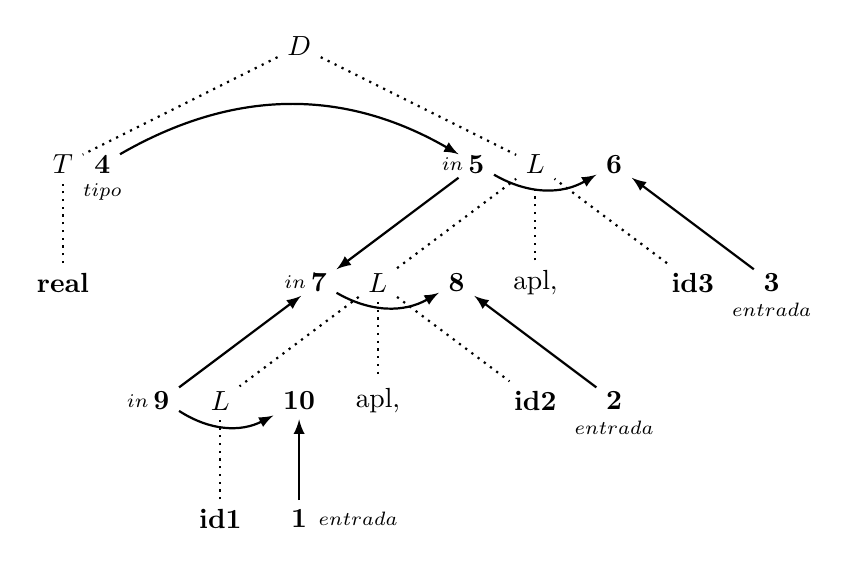
\begin{tikzpicture} 
            \node (A) at (6, 6) { $D$ };

            \node (B1) at (3, 4.5) { $T$ };
            \node (B2) at (9, 4.5) { $L$ };

            \node (X1) at (6, 0) { \textbf{1} };
            \node at (6.75, 0) { \scriptsize $entrada$ };
            \node (X2) at (10, 1.5) { \textbf{2} };
            \node at (10, 1.15) { \scriptsize $entrada$ };
            \node (X3) at (12, 3) { \textbf{3} };
            \node at (12, 2.65) { \scriptsize $entrada$ };
            \node (X4) at (3.5, 4.5) { \textbf{4} };
            \node at (3.5, 4.15) { \scriptsize $tipo$ };
            \node (X5) at (8.25, 4.5) { \textbf{5} };
            \node at (7.95, 4.5) { \scriptsize $in$ };
            \node (X6) at (10, 4.5) { \textbf{6} };
            \node (X7) at (6.25, 3) { \textbf{7} };
            \node at (5.95, 3) { \scriptsize $in$ };
            \node (X8) at (8, 3) { \textbf{8} };
            \node (X9) at (4.25, 1.5) { \textbf{9} };
            \node at (3.95, 1.5) { \scriptsize $in$ };
            \node (X10) at (6, 1.5) { \textbf{10} };

            \node (C1) at (3, 3) { \textbf{real} };
            \node (C2) at (7, 3) {  $L$ };
            \node (C3) at (9, 3) {  \code{apl}{,} };
            \node (C4) at (11, 3) {  \textbf{id3} };

            \node (D1) at (5, 1.5) { $L$ };
            \node (D2) at (7, 1.5) { \code{apl}{,} };
            \node (D3) at (9, 1.5) { \textbf{id2} };

            \node (E1) at (5, 0) { \textbf{id1} };

            \draw[thick,dotted] (A) to (B1);
            \draw[thick,dotted] (A) to (B2);
            \draw[thick,dotted] (C1) to (B1);
            \draw[thick,dotted] (C2) to (B2);
            \draw[thick,dotted] (C3) to (B2);
            \draw[thick,dotted] (C4) to (B2);
            \draw[thick,dotted] (C2) to (D1);
            \draw[thick,dotted] (C2) to (D2);
            \draw[thick,dotted] (C2) to (D3);
            \draw[thick,dotted] (E1) to (D1);

            \draw[-latex,thick] (X4) [bend left] to (X5);
            \draw[-latex,thick] (X5) [bend right] to (X6);
            \draw[-latex,thick] (X7) [bend right] to (X8);
            \draw[-latex,thick] (X9) [bend right] to (X10);
            \draw[-latex,thick] (X2) to (X8);
            \draw[-latex,thick] (X3) to (X6);
            \draw[-latex,thick] (X5) to (X7);
            \draw[-latex,thick] (X9) to (X7);
            \draw[-latex,thick] (X1) to (X10);
        \end{tikzpicture} 
    \end{figure}

\end{frame}

